
\section{Smith Chart}
\subsection{Eigenschaften}
	\begin{tabular}{p{10cm}p{8cm}}
		\begin{minipage}{10cm}
        	\begin{enumerate}{\setlength{\itemsep}{0cm}\setlength{\parsep}{0cm} \setlength{\topsep}{0cm}}
              \item \textbf{Normieren:} $Z_{\text{einzutragen}} = \frac{Z}{Z_0}$
              \item \textbf{Impedanz $\Leftrightarrow$ Admittanz:} Am Kreismittelpunkt spiegeln
              \item \textbf{Kurzschluss:} 	\textcolor{yellow}{Impedanz} \textcolor{orange}{Admittanz}
              \item \textbf{Leerlauf:}		\textcolor{orange}{Impedanz} \textcolor{yellow}{Admittanz}
        	  \item \textbf{Phase:}	Verlängerung der Reflexionsgerade an Kreisrand und Winkel ablesen
        	  \item \textbf{SWR:} Kreis mit Radius $|\Gamma|$ auf reeller Achse
        	  \item \textbf{Leitungslänge:} Äusserste Skala am Kreisrand  $\frac{l}{\lambda}$
        	  \item \textbf{Entnormieren:} $Z_{\text{gewünscht}} = Z_0
        	  Z_{\text{abgelesen}}$
            \end{enumerate}
        \end{minipage} &
		\begin{minipage}{8cm}
        	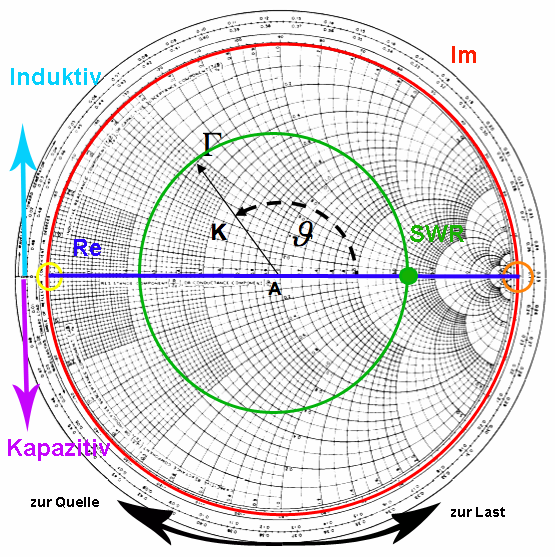
\includegraphics[height=7cm]{./images/SmithChart2.png}
        \end{minipage}
	\end{tabular}
\subsection{Formeln}
	$z=r+jx=\frac{1+\Gamma}{1-\Gamma}=\frac{1}{y}$ \qquad
	$\Gamma=\frac{z-1}{z+1}=\frac{1-y}{1+y}$
	
\subsection{Beispiele bei $Z_0=100\Omega$}
		\renewcommand{\arraystretch}{1.1}
		\begin{tabular}{| c | c | c | c | c | c |}
			\hline
				\textbf{Fall}
				& 1
				& 2 
				& 3
				& 4
				& 5 \\
			\hline
				\textbf{LE}
				& Anpassung
				& Leerlauf
				& Kurzschluss
				& $\lambda/8$ Stichleit. KS
				& $\lambda/8$ Stichleit. LL \\
			\hline
				\textbf{SWR}
				& 1
				& $\infty$
				& $\infty$
				& $\infty$
				& $\infty$ \\
			\hline
				\textbf{$\Gamma$}
				& $0$
				& $1 \angle 0 ^\circ$
				& $1 \angle 180 ^\circ$
				& $1 \angle 90 ^\circ$
				& $1 \angle 90 ^\circ$\\
			\hline
				\textbf{z}
				& $1+j0$
				& $\infty+j\infty$
				& $0+j0$
				& $0+j1$
				& $0-j1$ \\
			\hline
				\textbf{$v_{xm}$}
				& $-$
				& $\lambda/4$
				& $\lambda/2$
				& $3\lambda/8$
				& $\lambda/8$ \\
			\hline
				\textbf{Grafik}
				& 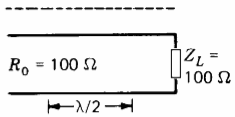
\includegraphics[height=0.9cm]{./images/Fall1.png}
				& 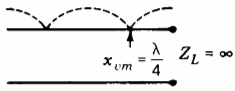
\includegraphics[height=0.9cm]{./images/Fall2.png}
				& 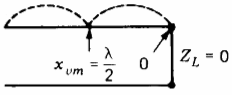
\includegraphics[height=0.9cm]{./images/Fall3.png}
				& 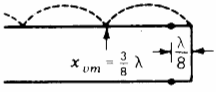
\includegraphics[height=0.9cm]{./images/Fall4.png}
				& 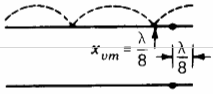
\includegraphics[height=0.9cm]{./images/Fall5.png} \\
			\hline
		\end{tabular}
		\renewcommand{\arraystretch}{1}
		